\chapter{Порядок Лоренца. Операции, ослабляющие и сохраняющие порядок. Взвешивание и смеси.}
\problem{} 
Стохастический порядок не сохраняется для премии Эсшера. Пример: совместное распределение двух рисков $X$ и $Y$ задается следующим образом при некотором $h > 0$:
$P(X = 0, Y = 0) = 1/3$, $P(X = 0, Y = 2/(3h)) = 1/3,$
$P(X = 3/h, Y = 3/h) = 1/3$.\\
Необходимо проверить, что $X <_{st} Y$, но $\Pi_X > \Pi_Y $.

\solution{}
    Премия Эсшера:
    \begin{equation}
        \Pi(X, h) = \Pi_X = \frac{\E\left[Xe^{hX}\right]}{g_X(h)} =  \frac{g'_X(h)}{g_X(h)}
    \end{equation}
    Из условия следуют совместные распределения $X$ и $Y$:
    \begin{figure*}[htbp]\label{hw07:task1tab1}
        \begin{tabular}{|c|c|c|}\hline
            $x$ & $0$ & $3/h$ \\\hline
            $P(X = x)$ & $2/3$& $1/3$  \\\hline
        \end{tabular}
        \begin{tabular}{cccc}
            &&&
        \end{tabular}
        \begin{tabular}{|c|c|c|c|}\hline
            $y$ & $0$ & $2/(3h)$ & $3/h$ \\\hline
            $P(Y = y)$ & $1/3$ &$1/3$&$1/3$\\\hline
        \end{tabular}
    \end{figure*}

    По определению стохастического порядка получаем, что $X <_{st} Y$ (см. рис. \ref{hw07:task1pic1}).
    \begin{figure}[htbp]
        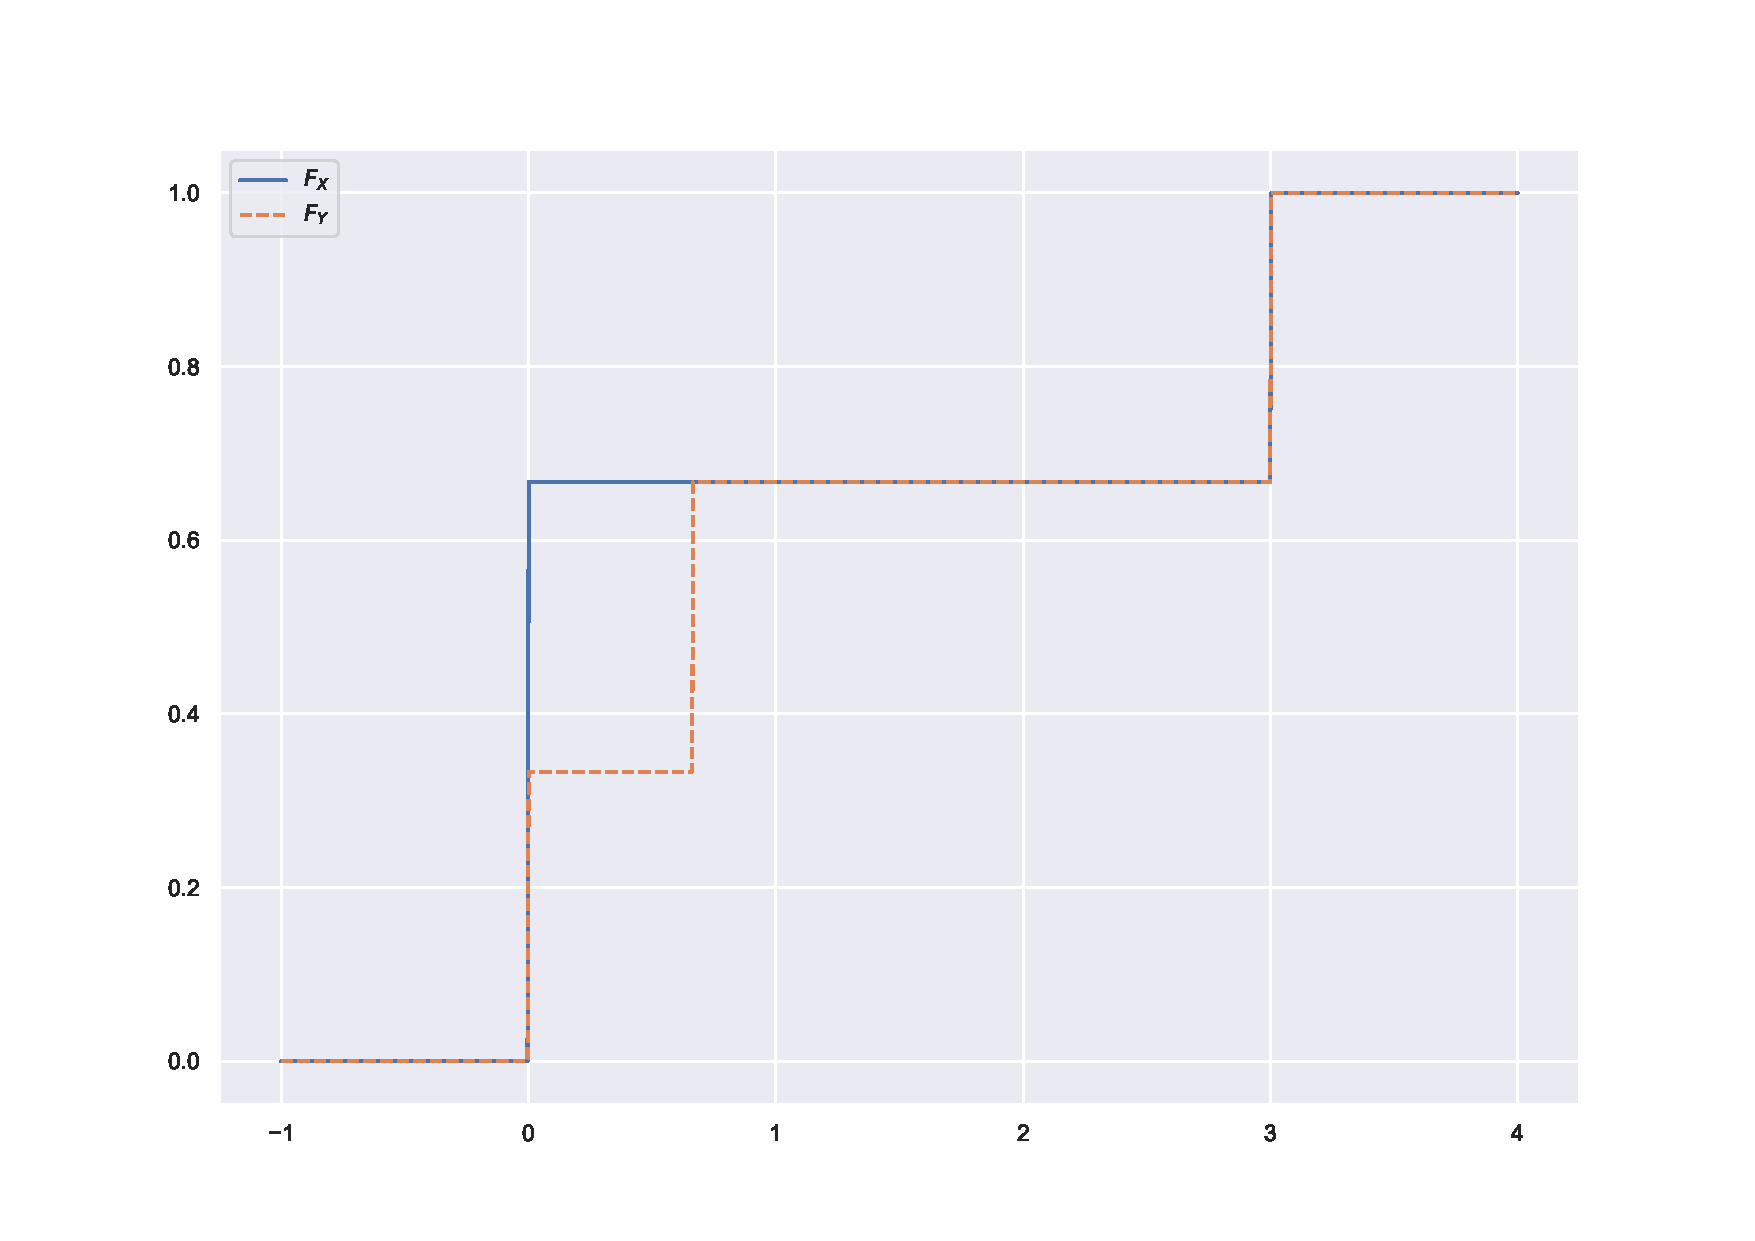
\includegraphics[width=\textwidth]{pics/hw7t1p1.pdf}\label{hw07:task1pic1}
        \caption{Функции распределения $X$ и $Y$}
    \end{figure}
    Теперь сравним соотвествующие премии:
    \begin{align}
        g_X(t) &= \frac{2}{3}+\frac{1}{3}e^{\frac{3}{h}t},  & g_X'(t) = \frac{1}{h}e^{\frac{3}{h}t};\\
        g_Y(t) &= \frac{1}{3}+\frac{1}{3}e^{\frac{3}{h}t} +\frac{1}{3}e^{\frac{2}{3h}t}, & g_Y'(t)=\frac{1}{h}e^{\frac{3}{h}t} +\frac{2}{9h}e^{\frac{2}{3h}t}.
    \end{align}
    Отсюда получаем
    \begin{align}
        \Pi_X &= \frac{\frac{1}{h}e^{3}}{\frac{2}{3}+\frac{1}{3}e^{\frac{3}{h}t}};\\
        \Pi_Y &= \frac{\frac{1}{h}e^{3} +\frac{2}{9h}e^{\frac{2}{3}}}{\frac{1}{3}+\frac{1}{3}e^{3} +\frac{1}{3}e^{\frac{2}{3}}}.
    \end{align}
    Посчитаем отношение премий:
    \begin{equation}
        \frac{\Pi_X}{\Pi_Y} \approx 1.02091201055381,
    \end{equation}
    что означает, что $\Pi_X > \Pi_Y$.


\problem{} Сохраняется ли стохастический порядок рисков при подсчете премий по принципу среднего квадратичного?

\solution{}
    Премия, посчитанная по принципу среднего квадратичного:
    \begin{equation}
        H(X) = \E\left[X\right] + \beta \std X.
    \end{equation}
    Пусть $X\sim Be(0.5)$, $Y\equiv 1$, $\beta = 2$. Тогда
    \begin{itemize}
        \item $\E\left[X\right] = 0.5$, $\std X = 0.5$, $H(X) = 1.5$;
        \item $\E\left[Y\right] = 1$, $\std Y = 0$, $H(Y) = 1$. 
    \end{itemize}
    Но $X<_{st}Y$. Значит, не сохраняется.

\problem{} Всегда ли принцип нулевой полезности обеспечивает премию с нагрузкой?

\solution{}
    Пусть экономический агент обладает склонностью к риску ($MU(x)$ не убывает). Тогда его функция полезности будет выпуклой. По неравенству Йенсена имеем
    \begin{equation}\label{hw07:task3eq1}
        \E\left[U(X)\right] \geq U\left(\E\left[X\right]\right).
    \end{equation}
    Премия, рассчитанная по принципу нулевой полезности, будет равна
    \begin{equation}\label{hw07:task3eq2}
        P\colon \quad \E\left[U(P-X)\right] = U(0).
    \end{equation}
    Из уравнений \eqref{hw07:task3eq1} и \eqref{hw07:task3eq2} следует, что
    \begin{equation}
        U(0) = \E\left[U(P-X)\right] \geq U\left(\E\left[P-X\right]\right) = U\left(P-\E\left[X\right]\right)
    \end{equation}
    Из монотонности полезности имеем, что 
    \begin{equation}
        0\geq P-\E\left[X\right] \implies P\leq\E\left[X\right]. 
    \end{equation}
    Поэтому эта премия не будет обеспечивать нагрузку.

\problem{} 
Как меняется в смысле порядка $<_e$ семейство показательных распределений при росте параметра?

\solution{}
    По определению: $X\leq_eY$, если $\forall \alpha > 0 \quad \E\left[e^{\alpha X}\right] \leq \E\left[e^{\alpha Y}\right]$.
    \begin{equation}
        \MGF(\alpha) = \begin{cases}
            \frac{\lambda}{\alpha-\lambda} & \alpha < \lambda, \\
            \infty & \alpha \geq \lambda.
        \end{cases}
    \end{equation}
    Очевидно, что по обоим аргументам функция строго монотонна на области определения. Поэтому экспоненциальный порядок сохраняет порядок на параметрах экспоненциального распределения.

\problem{} Экспоненциальный порядок не является полным порядком. Пример: $X$ имеет экспоненциальное распределение с
параметром $1$, а $Y$ - это смесь двух распределений, сосредоточенного в нуле и экспоненциального с параметром $1/2$, веса равны
соответственно $2/3$ и $1/3$. Проверить, что нельзя упорядочить указанные величины в смысле экспоненциального порядка.

\solution{}
    \begin{equation}
        \MGF_X(\alpha) = \begin{cases}
            \frac{1}{1-\alpha} & \alpha < 1, \\
            \infty & \alpha \geq 1.
        \end{cases}
    \end{equation}
    \begin{equation}
        \MGF_Y(\alpha) =\begin{cases}
            \frac{2}{3} + \frac{1}{3-6\alpha} & \alpha < \frac{1}{2}, \\
            \infty & \alpha \geq \frac{1}{2}.
        \end{cases}
    \end{equation}
    \begin{figure}[htbp]
        \begin{tabular}{|c|c|c|}\hline
              & $\MGF_X$ & $\MGF_Y$ \\\hline
            $\MGF$ & $\frac{1}{\alpha-1}$ & $\frac{2}{3} + \frac{1}{3- 6\alpha}$ \\\hline
            $\alpha = 1/6$ & $6/5$ & $7/6$ \\\hline
            $\alpha = 1/3$ & $3/2$ & $5/3$\\\hline
        \end{tabular}
    \end{figure}
    Отсюда видим, что распределения несравнимы в экспоненциальном смысле.